\documentclass[12pt]{article}
\usepackage{epsfig,a4}
%\usepackage{draftcopy}
\begin{document}
\thispagestyle{empty}
\title{CloudMan: project description Update 2}
\author{CERN IT-DEP/PES-PS}
%\version{0.1}
\date{\today}
\maketitle 
\begin{abstract}
\end{abstract}

\tableofcontents
\listoffigures 

\section{Scope of the project} 
The purpose of this project is the creation or adaption of a high level generic graphical management portal for IT resources.
The portal with working code name CloudMan, consists of a graphical web front-end, and several plugable back-ends. 

It has to be noted that the aim of this project is not to create another management console for virtual machine provisioning systems. These
are typically delivered with the provisioning systems themselves, and are still used to do the micro-management of these specific services.
The new tool is rather an abstract layer spanning over such installations, allowing automated and centralized configuration of resources at 
a high level, without looking into the details.

The architecture is shown in fig.~\ref{architecture}

\begin{figure}
\begin{center}
\includegraphics[width=0.9\textwidth]{architecture.eps}
\caption{\label{architecture} Basic architecture of the desired system. Users connect to the front-end which offers a graphical user interface. They authenticate using the site Single Sign On mechanism or similar. The data which is entered is stored in an external database, and exported in a low level format. Back-ends which are design to configure specific services, for example local cloud installations, consume this information to configure their resources.}
\end{center}
\end{figure}


\subsection{Front-end}
The front-end consists of a graphical user interface which is used to enter configuration data. It will export the entered information 
in a machine readable form~\footnote{XML or similar}, which can then be consumed by different back-ends interfacing to IT services.

The front-end 
\begin{itemize}
\item will provide a single entry point for the site resource manager to manage resources for large user communities such as virtual organization (VO)~\footnote{A user community can be a Virtual Organization, or an equivalent entity, for example a HEP experiment.}. 
\item will allow the allocation of existing hardware resources to different projects
\end{itemize}

 
\subsection{Back-ends}
The configuration data exported by the front-end is consumed by one or more back-ends. These back-ends are service specific, and will consume only
this part of the data which are relevant to configure the specific service, for example resources for an internal cloud, or resources for 
virtualized services. 

Back-ends will be service specific, and can be site specific. 

The tool is designed to cover a high level overview over resource allocations for different communities who use the services offered by IT, and will be flexible enough to spread over different regions, thus allowing to remotely manage resources of off-site installations (key word: remote hosting).

In the case of back-ends interfacing to cloud or virtualization services, the detailed configuration of the actual hardware is left to the orchestrator in use. The orchestrators are left to sort out the tactical allocation such as least loaded hypervisors. The back-end is only used to configure such orchestrators. 

\section{Definitions}
Details on the following definitions are described in the design document.

\subsection{Regions}
\begin{itemize}
\item A region describes the a physical location of resources, for example CERN/Meyrin. 
\item It can consist of zero or more zones.
\item It has a name and a description.
\item It is managed by one or more administrators (an e-group).
\end{itemize}

\subsection {Resources}
\begin{itemize}
\item It is a set of entities (machines) on which computations can be done.
\item The capability of a resource is measured on the basis of four different metrics:
\begin{itemize}
\item Computational capacity (hepspecs)
\item Memory Size
\item Storage Capacity
\item Network Bandwidth 
\end{itemize}
\item Every resource has a resource class attribute specifying whether the resource is physical or virtual.
\end{itemize}

\subsection {Resource Types}
\begin{itemize}
\item A resource type is a template of resources. It is something from which an actual resource can be instantiated.
\item Each resource type has a total capacity in terms of CPU, memory, storage and bandwidth.
\item A resource type may either contain physical resources or virtual resources but not both. This is highlighted by the resource class attribute.
\end{itemize} 

\subsection{Zones}
\begin{itemize}
\item A zone is a subset of a region. A zone belongs to only one region.
\item It describes a set of resources at a specific region with specific features.
\item Zones within a region can have different specific features, for example in terms of networking or redundancies, reflected in the hardware layout.
\item Each zone has a total capacity which is expressed in terms of CPU, memory, storage and bandwidth.
\item Each zone has a name and a description.
\item In each zone, there is a set of allowed resource types. The zone may consist of only the resources belonging to the allowed resource types.
\item Zones are maintained by administrators (e-groups). These administrators can be same as the a 
\end{itemize}

\subsection{User communities/ Groups}
A user community is a top level group of users, such as a VO or an experiment~\footnote{for example ATLAS or CMS}
\begin{itemize}
\item A group is a collection of users, who share some common characteristics. This common characteristic could be - an experiment in which they are involved, the host institution to which they belong etc.
\item A group has a name and a description.
\item The group members are part of an e-group.
\item There may be parent-child relationships among groups. But those are ignored by CloudMan and these relationships are not a part of the schema. This information is present in the CERN e-groups.
\end{itemize}

\subsection{Projects}
A project is a high level configuration entity which consists of
\begin{itemize}
\item a list of services
\item a project administrator (group), see below
\end{itemize}
A project has a name and a description. There may be other administrator defined metadata in a project.

\subsection{Roles}
Roles are defined in a strictly hierarchical manner, the resource manager being the most powerful user, and a normal user being the least powerful user with restricted access to information. This is shown in fig.~\ref{pyramide}.

\begin{figure}
\begin{center}
\includegraphics[width=0.8\textwidth]{pyramide.eps}
\caption{\label{pyramide} Hierarchical order of roles. The lower the power the more people can have the role. The most powerful user is the resource manager. Ideally, this is a single individual, eventually complemented by a backup. Normal users can be any registered user, which can be many thousands.}
\end{center}
\end{figure}
 
\subsubsection{Resource manager}
The resource manager is a person or a small group of people who have administrative privileges with the right to allocate resources to a VO, projects and services. 

\begin{figure}
\begin{center}
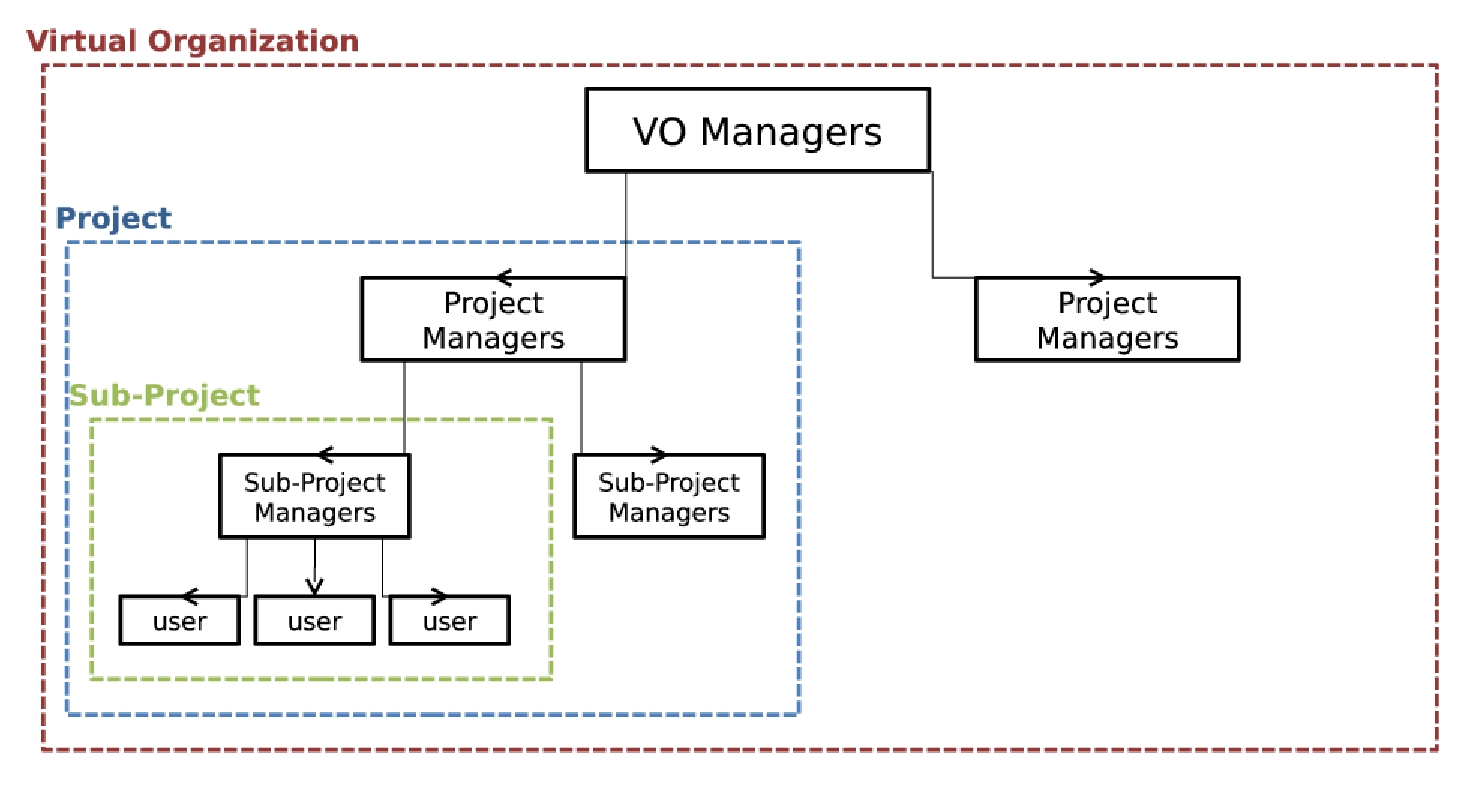
\includegraphics[width=0.8\textwidth]{vo_roles.eps}
\caption{\label{vo_roles} Hirarchies within VOs: Each VO has one or more VO manager who approves the different projects within the VO, nominates project managers and so forth. The project managers, in turn, can manage different sub-projects which belong to the project they manage. Users don't have special rights. They are part of a sub-project in which they work. 
}
\end{center}
\end{figure}


Resource allocations by the resource manager are done in absolute values. 
\begin{itemize}
\item the resource manager ensures that the requested resources match the available resources in the resource pools
\item the resource manager ensures that resources in the resource pools are not over-committed
\end{itemize}
The resource managers job is of a high level strategic nature. His main task is to allocate large chunks of resources to a VO, and set quotas. 

\subsubsection{VO manager}
A VO manager is a person or a group of persons with administrative privileges within the group they belong to. They can define projects and do free resource allocations within the allocations made to their VO. The VO manager also owns and manages the project manager lists. 

\subsubsection{Project manager}
A project manager is a person or a group of persons with administrative privileges for a specific project. They can define services withing their project, and do free resource allocations to the services belonging to this project, within the limits of the total resource allocations for the project. 

\subsubsection{Normal users}
A normal user is a user of the portal who can browse certain contents of the site. Only authenticated users are allowed to access the portal. ACLs are determined by the VO and the role of the user within this VO to which the user belongs. There is no anonymous user concept foreseen. 
Specifically, if a user successfully authenticates but does not belong to any of the supported VOs, access to VO specific information will be restricted.

\subsection{Resource pools}
\begin{figure}
\begin{center}
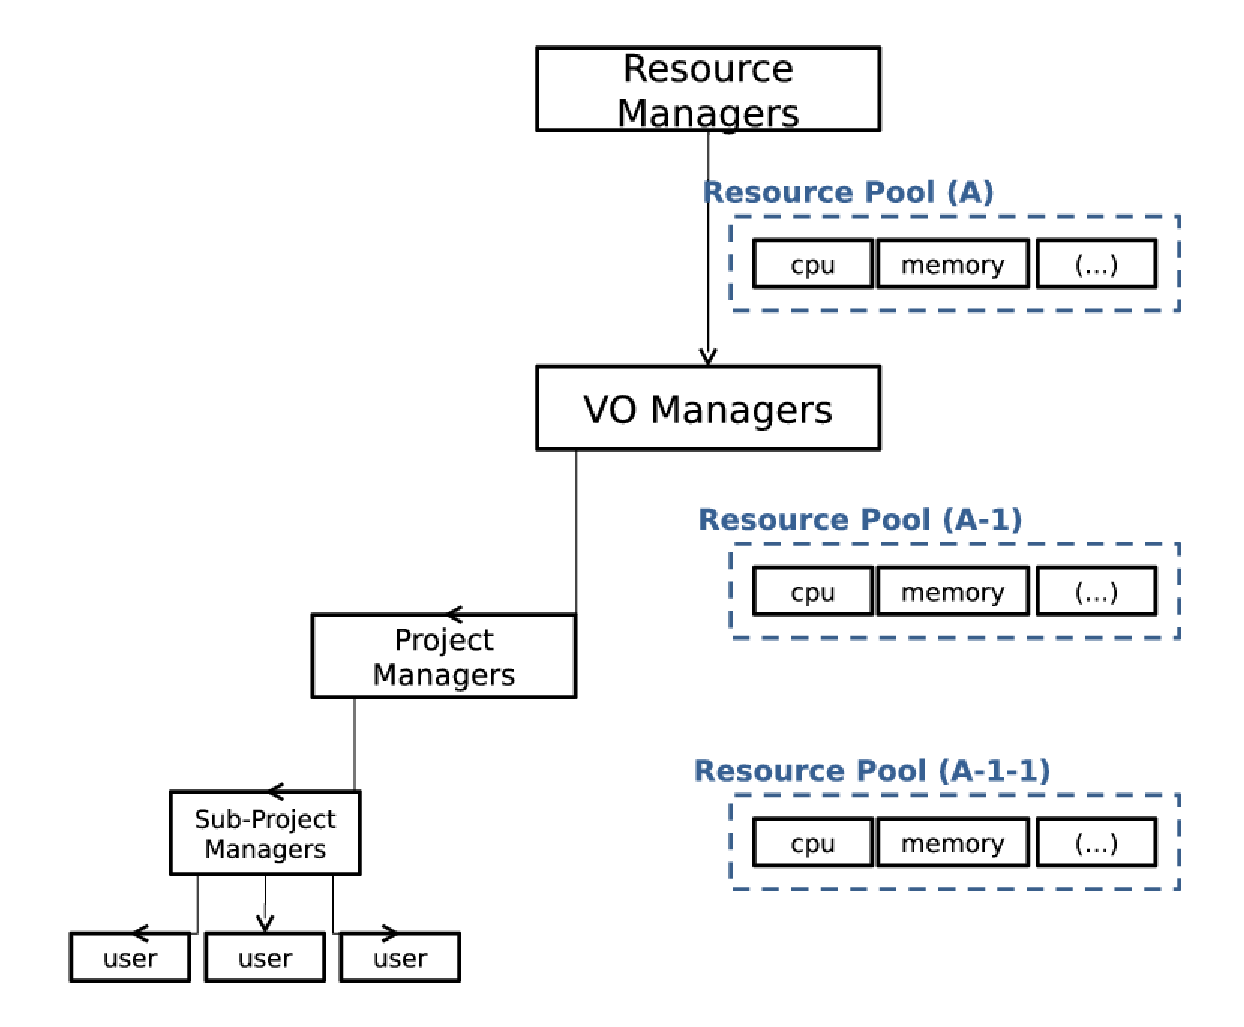
\includegraphics[width=0.7\textwidth]{roles.eps}
\caption{\label{roles} Relationship between roles and resource pools. The resource manager has an abstract high level view over available resource pools. He allocates fractions of these resource pools to VO managers who can in turn allocate bits of these resource pools to the different projects, and so forth. 
}
\end{center}
\end{figure}
A resource pool is a pool of different resources (CPU, disk, ...) with attributes which describe its nature. Required resource pool features include 
\begin{itemize}
\item A name for the pool
\item The region or the zone of the resource pool
\item Total amount of CPU, disk space,  memory
\item Network bandwidth
\item A list of underlying resource pools
\item A minimum number of job or VM slots. 
\item Support for life migration (for virtualized resources)
\item Support for migration (for virtualized resources)
\end{itemize}
The relationship between resource pools and the different roles is shown in fig.~\ref{roles}.

\section{Requirements}
\subsection{Required features}

\subsubsection{General requirements}
\begin{itemize}
\item The use of the tool is not restricted to a single region. It will support the configuration of several computer 
centers which belong to the same organization. As an example, CERN has resources at the Meyrin site and resources hosted externally at Geneva~\footnote{Weather or not these regions are managed together or inside different resource pools is a configuration choice}.
\item All code must make use of standard, non proprietary formats, scripting and programming languages, to ensure that it will be easy to maintain
\item The front end is generic and uses high level information only. For example, it knows about total disk space, total CPU power etc. only. It has no knowledge of any implementation details, like host names, operating systems, ...
\item All state data has to be stored in a database
\item It must be possible to run this database remotely
\item The implementation should follow best practices. Any libraries and configuration files should be placed in standard locations, and system messages should be logged using syslog. 
\end{itemize}


\subsubsection{Configuration}
\begin{itemize}
\item There is no hard coded meta data information in the code. Any site specific configuration can be done via plain text or similar, machine and human readable configuration files.
\item It must be possible to entirely configure the tool using site configuration tools, namely Quattor~\cite{quattor}.
\item Flat text file configuration files should be used unless there is a good reason for more complex structures, like XML formatted configuration files. 
\end{itemize}

\subsubsection{Modularity}
\begin{itemize}
\item Users and groups of users (eg the different groups of managers) can be resolved via different methods
\item The methods are implemented as plugins
\item The initial implementation must support at least user lists, unix groups and LDAP
\item LDAP support is required. The role definition must be based on ldap groups.
\item LDAP support must be implemented in a way which allows to easily use CERN egroups via a simple configuration change
\item It must be possible to extend the system to eg disk resource allocations by simply editing a configuration file   
\item Both mysql and Oracle databases must be supported. Which one is determined when the tool is configured. 
\end{itemize}

\subsubsection{Access}
\begin{itemize}
\item Different authentication mechanisms must be supported: plain password, Kerberos5, Single-Sign-On
\item The system must work with CERN SSO for authentication
\item The tool must support different access models depending on the role individual users have. 
\item Access patterns are organized strictly hierarchical. 
\end{itemize}

\subsubsection{Security}
\begin{itemize}
\item Access to the configuration data provided by the front-end must be authenticated. The authenticity of the front-end must be checked, and the integrity of the provided data must be ensured.
\item No secret information (like passwords etc) must be configured and exported by the front end.
\end{itemize}

\subsection{Optional features}
Optional features are not required initially. They can be added at a later stage, after they have been reviewed.
\begin{itemize}
\item A feedback loop would be nice to have: back-ends report the current status of their resource usage. This information can be used by the 
front end to easy up the configuration. 
\item The tool is extended to configure not only CPU but also for example disc resources
\item The tool can be run as a load balanced service. Several instances can be hidden behind a single alias.
\end{itemize}

%
%
%
\section{Use cases}
\subsection{Resource manager}
The resource manager has several resource pools which can be located at different regions and zones within those regions, offering a fixed amount 
resources. 
\begin{itemize}
\item The resource manager approves new user communities (eg. VO). 
\item The resource manager deletes user communities, freeing all resources previously allocated to this user community.
\item The resource manager assigns resources to a user community. He does this depending on the available resource pools and their features.
\item the resource manager approves resource requests from VO managers for their VO
\item The resource manager changes the resource allocation to a user community. He can
 \begin{itemize}
   \item increase the allocation
   \item reduce the allocation 
   \item move allocation between resource pools, keeping the total allocation constant
 \end{itemize}
\end{itemize}


\subsection{VO manager}
The VO manager manages resource allocations for the VO he belongs to. Resource allocations for projects is done in a relative way. 
\begin{itemize} \item The VO manager approves new project requests
\item The VO manager denies new projects requests
\item The VO manager manages project manager lists for already existing and approved projects
\item The VO manager changes the total project resource allocations
\item the VO manager approves resource requests for projects within his group allocation
\item the VO manager requests resources for his project 
  \begin{itemize}
    \item increase the allocation of a resource pool allocation to a project
    \item reduce the allocation  of a resource pool allocation to a project
    \item move allocation between resource pools, keeping the total allocation constant
  \end{itemize}
\end{itemize}

\subsection{Project manager}
The project manager manages his projects. 
\begin{itemize}
\item the project manager requests a new project 
\item the project manager defines sub-projects for his projects
\item the project manager approves sub-project requests 
\item the project manager approves sub-project managers
\item the project manager can define sub-project managers 
\item the project manager approves resource requests for sub-projects within his project
\item the project manager requests resource for his project within the VO allocation
\item the project manager assigns resources to the sub-projects of his projects
\item the project manager changes project resource allocations by 
  \begin{itemize}
    \item increasing the allocation of a resource pool allocation to a sub-project
    \item reducing the allocation  of a resource pool allocation to a sub-project
    \item moving the allocation between resource pools, keeping the total allocation constant
  \end{itemize}
\end{itemize}

\subsection{Users}
A user here is a normal user without any privileges. 
\begin{itemize}
\item A user logs in and browses the information. He belongs to a certain VO, 
and will only see information which is relevant for the VO he belongs to.
\item A user logs in and tries to change something. His changes are not accepted.  
\item A user requests a project within the VO he belongs to.
\item A user requests a sub-project to a project he's a member of already.
\end{itemize}
In practice, a user can belong to different VOs. In the early phases of this project, only one VO per user will be supported. At a later stage of the project, authentication may be extended to certificates. The subject of the certificate the user presents may identify his role and the VO he belongs to.

\subsection{General use cases}
\begin{itemize}
\item A new region is created. New resources come in and are allocated to existing groups.
\item A new VO comes into the game, and requests allocation of resources
\item An existing VO wants to shift their main activity from local batch processing to batch processing
\item An existing VO wants to shift their resources from batch processing to a self service infrastructure
\item An existing VO wants to make use of an hybrid cloud, and ask for additional resources
\item An existing VO decides to move away from the grid and use VOBoxes instead
\item An existing VO wants to know the fraction of their grid/local batch/self-service/cloud usage
\end{itemize}

\section{Additional Test cases}
\begin{itemize}
\item The system can be configured to use CERN e-groups (via LDAP). 
\item CERN users authenticate via SSO, and get mapped to the proper role they have as defined by an e-group (via LDAP).
\item Authenticated users can only access and change the information which corresponds to their role.
\end{itemize}

\section{Phases}

The project has three phases. Each phase starts with a review of the existing infrastructure, and learn of experiences to improve the tool.
 
\subsection{Phase 1}
For the first phase, CERN-IT will provide a detailed project description and project design, which will be
discussed with representatives of all participating parties. Part of this phase is a survey of possibly existing tools which 
may cover most of the use cases. 
It has to be evaluated if such a tool can be extended to match our needs, in case it exists, and go for a full implementation otherwise.

Milestones for this phase include:
\begin{itemize}
\item a project description document
\item a detailed project design document
\item a working front end which covers the use cases 
\item at least one back-end to configure services. The first back-end to implement should be usable to configure a cloud management system, 
for example OpenNebula~\cite{ONE}. 
\item a sample implementation for back-ends which can be used by other service managers to configure their services using the new tool
\end{itemize}

\subsection{Phase 2}
The second phase should cover 
\begin{itemize}
\item bug fixes for the product resulting from the first phase
\item feature requests from the first operational experiences
\item an updated design document driving the second phase, which covers all feature requests and requests for enhancements so far
\end{itemize}

Milestones for this phase include:
\begin{itemize}
\item an updated detailed project design document
\item a production quality front-end tool
\item a production ready back-end to configure internal clouds 
\end{itemize}

\subsection{Phase 3}
The third phase covers another cycle of bug fixes and feature request treatment. It is dedicated for production release and operations. 
Milestones for this phase include:
\begin{itemize}
\item The tool is used to configure production services, eventually replacing already existing tools 
\end{itemize}



\begin{thebibliography}{99}
\bibitem{ONE}
See: http://opennebula.org
%\bibitem{ISF}
%http://www.platform.com/private-cloud-computing/private-cloud-platform-isf
%\bibitem{AC}
%http://www.platform.com/private-cloud-computing/hpc-clou
%\bibitem{LSF}
%Release Notes for Platform LSF Version 7.0, Nov. 2006,  PLATFORM corporation.
%\bibitem{XEN}
%http://www.xen.org
%\bibitem{KVM}
%http://www.linux-kvm.org
\bibitem{quattor}
http://www.quattor.org
\end{thebibliography}
\end{document}


